% questions.tex —— 2005 年·普通高等学校招生考试·江苏卷 · 题目内容片段（无答案）
% 由 tools/generate_projects.py 依来源总账自 2005/2005_数学真题_江苏_试题.md 生成，勿手改（改源 MD 后重跑）

\begin{question}
\gkti{1}设集合 $A = \{1, 2\}$，$B = \{1, 2, 3\}$，$C = \{2, 3, 4\}$，则 $(A \cap B) \cup C =$\mbox{（　　）}

\begin{gkopts}(4)
\task A．$\{1, 2, 3\}$
\task B．$\{1, 2, 4\}$
\task C．$\{2, 3, 4\}$
\task D．$\{1, 2, 3, 4\}$
\end{gkopts}

\end{question}
\begin{question}
\gkti{2}函数 $y = 2^{1-x} + 3\ (x \in \mathbf{R})$ 的反函数的解析表达式为\mbox{（　　）}

\begin{gkopts}(2)
\task A．$y = \log_2 \dfrac{2}{x-3}$
\task B．$y = \log_2 \dfrac{x-3}{2}$
\task C．$y = \log_2 \dfrac{3-x}{2}$
\task D．$y = \log_2 \dfrac{2}{3-x}$
\end{gkopts}

\end{question}
\begin{question}
\gkti{3}在各项都为正数的等比数列 $\{a_n\}$ 中，首项 $a_1 = 3$，前三项和为 $21$，则 $a_3 + a_4 + a_5 =$\mbox{（　　）}

\begin{gkopts}(4)
\task A．$33$
\task B．$72$
\task C．$84$
\task D．$189$
\end{gkopts}

\end{question}
\begin{question}
\gkti{4}在正三棱柱 $ABC - A_1B_1C_1$ 中，若 $AB = 2$，$AA_1 = 1$，则点 $A$ 到平面 $A_1BC$ 的距离为\mbox{（　　）}

\begin{gkopts}(2)
\task A．$\dfrac{\sqrt{3}}{4}$
\task B．$\dfrac{\sqrt{3}}{2}$
\task C．$\dfrac{3\sqrt{3}}{4}$
\task D．$\sqrt{3}$
\end{gkopts}

\end{question}
\begin{question}
\gkti{5}$\triangle ABC$ 中，$A = \dfrac{\pi}{3}$，$BC = 3$，则 $\triangle ABC$ 的周长为\mbox{（　　）}

\begin{gkopts}(1)
\task A．$4\sqrt{3}\sin\left(B + \dfrac{\pi}{3}\right) + 3$
\task B．$4\sqrt{3}\sin\left(B + \dfrac{\pi}{6}\right) + 3$
\task C．$6\sin\left(B + \dfrac{\pi}{3}\right) + 3$
\task D．$6\sin\left(B + \dfrac{\pi}{6}\right) + 3$
\end{gkopts}

\end{question}
\begin{question}
\gkti{6}抛物线 $y = 4x^2$ 上的一点 $M$ 到焦点的距离为 $1$，则点 $M$ 的纵坐标是\mbox{（　　）}

\begin{gkopts}(4)
\task A．$\dfrac{17}{16}$
\task B．$\dfrac{15}{16}$
\task C．$\dfrac{7}{8}$
\task D．$0$
\end{gkopts}

\end{question}
\begin{question}
\gkti{7}在一次歌手大奖赛上，七位评委为歌手打出的分数如下：$9.4$，$8.4$，$9.4$，$9.9$，$9.6$，$9.4$，$9.7$．去掉一个最高分和一个最低分后，所剩数据的平均值和方差分别为\mbox{（　　）}

\begin{gkopts}(4)
\task A．$9.4$，$0.484$
\task B．$9.4$，$0.016$
\task C．$9.5$，$0.04$
\task D．$9.5$，$0.016$
\end{gkopts}

\end{question}
\begin{question}
\gkti{8}设 $\alpha$，$\beta$，$\gamma$ 为两两不重合的平面，$l$，$m$，$n$ 为两两不重合的直线，给出下列四个命题：

① 若 $\alpha \perp \gamma$，$\beta \perp \gamma$，则 $\alpha \parallel \beta$；

② 若 $m \subset \alpha$，$n \subset \alpha$，$m \parallel \beta$，$n \parallel \beta$，则 $\alpha \parallel \beta$；

③ 若 $\alpha \parallel \beta$，$l \subset \alpha$，则 $l \parallel \beta$；

④ 若 $\alpha \cap \beta = l$，$\beta \cap \gamma = m$，$\gamma \cap \alpha = n$，$l \parallel \gamma$，则 $m \parallel n$．

其中真命题的个数是\mbox{（　　）}

\begin{gkopts}(4)
\task A．$1$
\task B．$2$
\task C．$3$
\task D．$4$
\end{gkopts}

\end{question}
\begin{question}
\gkti{9}设 $k = 1, 2, 3, 4, 5$，则 $(x + 2)^5$ 的展开式中 $x^k$ 的系数不可能是\mbox{（　　）}

\begin{gkopts}(4)
\task A．$10$
\task B．$40$
\task C．$50$
\task D．$80$
\end{gkopts}

\end{question}
\begin{question}
\gkti{10}若 $\sin\left(\dfrac{\pi}{6} - \alpha\right) = \dfrac{1}{3}$，则 $\cos\left(\dfrac{2\pi}{3} + 2\alpha\right) =$\mbox{（　　）}

\begin{gkopts}(4)
\task A．$-\dfrac{7}{9}$
\task B．$-\dfrac{1}{3}$
\task C．$\dfrac{1}{3}$
\task D．$\dfrac{7}{9}$
\end{gkopts}

\end{question}
\begin{question}
\gkti{11}点 $P(-3, 1)$ 在椭圆 $\dfrac{x^2}{a^2} + \dfrac{y^2}{b^2} = 1\ (a > b > 0)$ 的左准线上．过点 $P$ 且方向为 $\vec{a} = (2, -5)$ 的光线，经直线 $y = -2$ 反射后通过椭圆的左焦点，则这个椭圆的离心率为\mbox{（　　）}

\begin{gkopts}(2)
\task A．$\dfrac{\sqrt{3}}{3}$
\task B．$\dfrac{1}{3}$
\task C．$\dfrac{\sqrt{2}}{2}$
\task D．$\dfrac{1}{2}$
\end{gkopts}

\end{question}
\begin{question}
\gkti{12}四棱锥的 $8$ 条棱代表 $8$ 种不同的化工产品，有公共点的两条棱代表的化工产品放在同一仓库是危险的，没有公共顶点的两条棱代表的化工产品放在同一仓库是安全的，现打算用编号为①、②、③、④的 $4$ 个仓库存放这 $8$ 种化工产品，那么安全存放的不同方法种数为\mbox{（　　）}

\begin{gkopts}(4)
\task A．$96$
\task B．$48$
\task C．$24$
\task D．$0$
\end{gkopts}

\end{question}
\begin{question}
\gkti{13}命题“若 $a > b$，则 $2^a > 2^b - 1$”的否命题为＿＿＿＿＿＿．

\end{question}
\begin{question}
\gkti{14}曲线 $y = x^3 + x + 1$ 在点 $(1, 3)$ 处的切线方程是＿＿＿＿＿＿．

\end{question}
\begin{question}
\gkti{15}函数 $y = \sqrt{\log_{0.5}(4x^2 - 3x)}$ 的定义域为＿＿＿＿＿＿．

\end{question}
\begin{question}
\gkti{16}若 $3^a = 0.618$，$a \in [k, k+1)$，$k \in \mathbf{Z}$，则 $k =$＿＿＿＿＿＿．

\end{question}
\begin{question}
\gkti{17}已知 $a$，$b$ 为常数，若 $f(x) = x^2 + 4x + 3$，$f(ax + b) = x^2 + 10x + 24$，则 $5a - b =$＿＿＿＿＿＿．

\end{question}
\begin{question}
\gkti{18}在 $\triangle ABC$ 中，$O$ 为中线 $AM$ 上的一个动点，若 $AM = 2$，则 $\overrightarrow{OA} \cdot \left(\overrightarrow{OB} + \overrightarrow{OC}\right)$ 的最小值是＿＿＿＿＿＿．

\Needspace{0.4\textheight}
\end{question}
\begin{question}
\gkti{19}如图，圆 $O_1$ 与圆 $O_2$ 的半径都是 $1$，$O_1O_2 = 4$，过动点 $P$ 分别作圆 $O_1$、圆 $O_2$ 的切线 $PM$、$PN$（$M$、$N$ 分别为切点），使得 $PM = \sqrt{2}\,PN$．试建立适当的坐标系，并求动点 $P$ 的轨迹方程．
\nopagebreak[4]
\begin{center}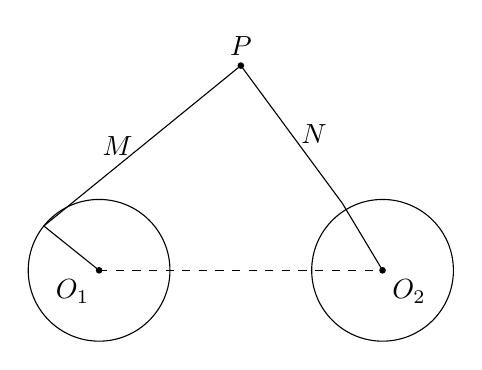
\begin{tikzpicture}[scale=1.0]
  \draw (0,0) circle (0.9);
  \draw (3.6,0) circle (0.9);
  \fill (0,0) circle (1.2pt) node[below left] {$O_1$};
  \fill (3.6,0) circle (1.2pt) node[below right] {$O_2$};
  \draw[dashed] (0,0) -- (3.6,0);
  \coordinate (P) at (1.8,2.6);
  \coordinate (M) at (-0.702,0.563);
  \coordinate (N) at (3.09,0.85);
  \draw (P) -- (M) node[midway, left] {$M$};
  \draw (P) -- (N) node[midway, right] {$N$};
  \fill (P) circle (1.2pt) node[above] {$P$};
  \draw (M) -- (0,0);
  \draw (N) -- (3.6,0);
\end{tikzpicture}
\end{center}
\nopagebreak[4]
\end{question}
\begin{question}
\gkti{20}甲、乙两人各射击一次，击中目标的概率分别是 $\dfrac{2}{3}$ 和 $\dfrac{3}{4}$．假设两人射击是否击中目标，相互之间没有影响；每次射击是否击中目标，相互之间没有影响．

(1) 求甲射击 $4$ 次，至少 $1$ 次未击中目标的概率；

(2) 求两人各射击 $4$ 次，甲恰好击中目标 $2$ 次且乙恰好击中目标 $3$ 次的概率；

(3) 假设某人连续 $2$ 次未击中目标，则停止射击．问：乙恰好射击 $5$ 次后，被中止射击的概率是多少？

\Needspace{0.4\textheight}
\end{question}
\begin{question}
\gkti{21}如图，在五棱锥 $S - ABCDE$ 中，$SA \perp$ 底面 $ABCDE$，$SA = AB = AE = 2$，$BC = DE = \sqrt{3}$，$\angle BAE = \angle BCD = \angle CDE = 120^\circ$．

(1) 求异面直线 $CD$ 与 $SB$ 所成的角（用反三角函数值表示）；

(2) 证明：$BC \perp$ 平面 $SAB$；

(3) 用反三角函数值表示二面角 $B - SC - D$ 的大小（本小问不必写出解答过程）．
\nopagebreak[4]
\begin{center}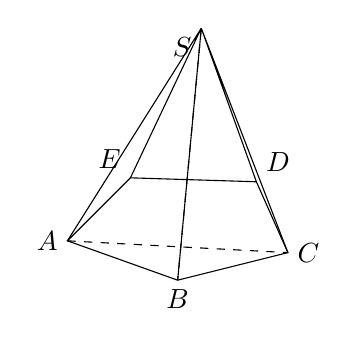
\begin{tikzpicture}[scale=1.0]
  \coordinate (S) at (0.4,2.5);
  \coordinate (A) at (-1.3,-0.2);
  \coordinate (B) at (0.1,-0.7);
  \coordinate (C) at (1.5,-0.35);
  \coordinate (D) at (1.1,0.55);
  \coordinate (E) at (-0.5,0.6);
  \draw (S) -- (A) (S) -- (B) (S) -- (C) (S) -- (D) (S) -- (E);
  \draw (A) -- (B) -- (C) -- (D) -- (E) -- cycle;
  \draw[dashed] (S) -- (B);
  \draw[dashed] (A) -- (C);
  \node[below left] at (S) {$S$};
  \node[left] at (A) {$A$};
  \node[below] at (B) {$B$};
  \node[right] at (C) {$C$};
  \node[above right] at (D) {$D$};
  \node[above left] at (E) {$E$};
\end{tikzpicture}
\end{center}
\nopagebreak[4]
\end{question}
\begin{question}
\gkti{22}已知 $a \in \mathbf{R}$，函数 $f(x) = x^2|x - a|$．

(1) 当 $a = 2$ 时，求使 $f(x) = x$ 成立的 $x$ 的集合；

(2) 求函数 $y = f(x)$ 在区间 $[1, 2]$ 上的最小值．

\end{question}
\begin{question}
\gkti{23}设数列 $\{a_n\}$ 的前 $n$ 项和为 $S_n$，已知 $a_1 = 1$，$a_2 = 6$，$a_3 = 11$，且
\nopagebreak[4]
\[
(5n - 8)S_{n+1} - (5n + 2)S_n = An + B,\quad n = 1, 2, 3, \cdots,
\]
其中 $A$，$B$ 为常数．

(1) 求 $A$ 与 $B$ 的值；

(2) 证明数列 $\{a_n\}$ 为等差数列；

(3) 证明不等式 $\sqrt{5a_{mn}} - \sqrt{a_m a_n} > 1$ 对任何正整数 $m$、$n$ 都成立．

\end{question}